\subsection{Caso d'uso UC1: Scenario principale}
\begin{center}
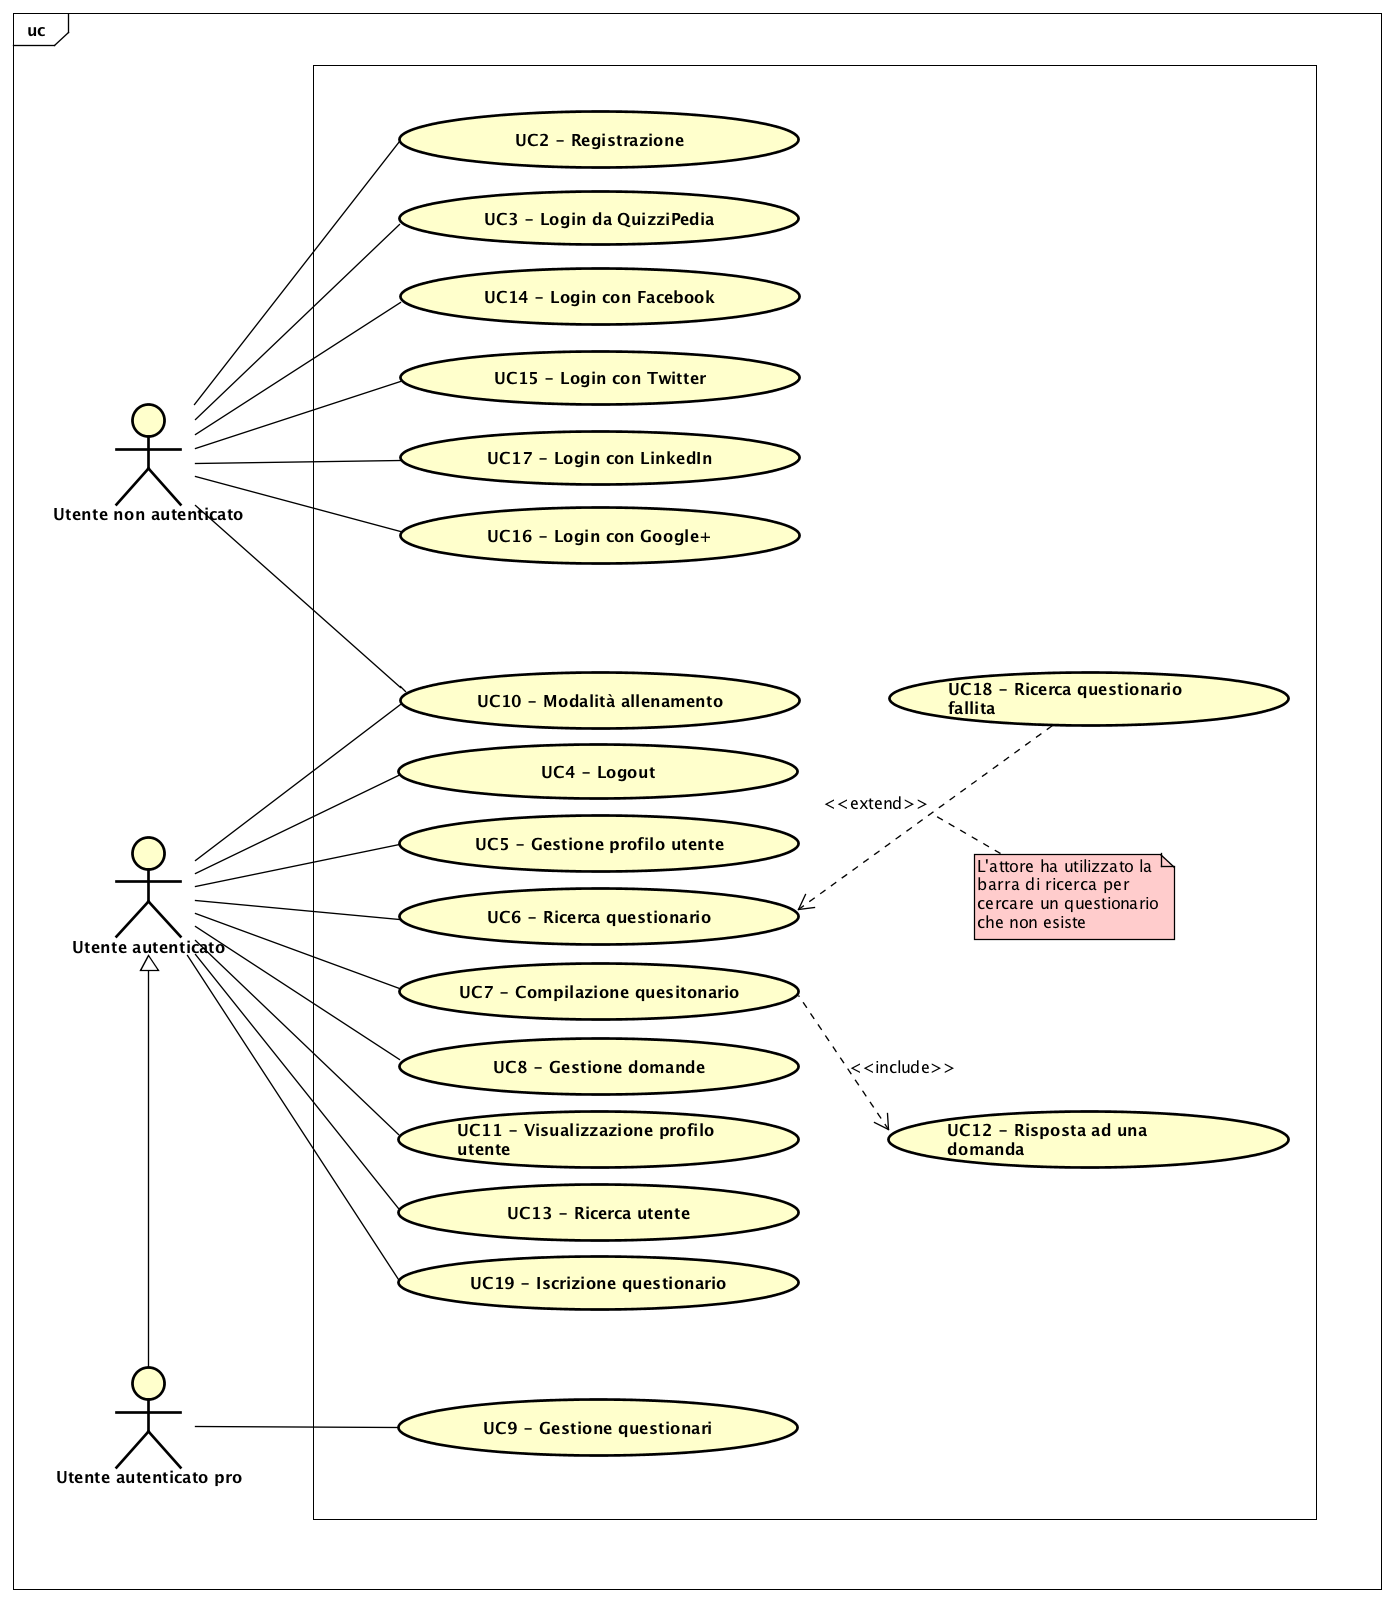
\includegraphics[scale=0.5]{UML/UC1.png}
\end{center}
\begin{itemize}
\item\textbf{Attori}: utente, utente autenticato, utente autenticato pro;
\item\textbf{Descrizione}: nella schermata principale un utente non autenticato può ricercare e compilare questionari pubblici esistenti. Può inoltre autenticarsi tramite l'apposito form di login oppure registrarsi.\\
L'utente autenticato, oltre a svolgere tutte le operazioni dell'utente non autenticato, è abilitato a:
\begin{itemize}
\item Effettuare il logout;
\item Gestire il proprio profilo: modificare il proprio nome, cognome, indirizzo e-mail e password. Può visualizzare i questionari realizzati, compilati e consultare le relative valutazioni ricevute;
\item Gestire le domande: inserire nuove domande nel sistema oppure eliminarne una da lui creata;
\item Gestire i questionari: creare questionari pubblici oppure eliminare un questionario da lui creato.
\end{itemize}

L'utente autenticato pro può, oltre a svolgere tutte le operazioni dell'utente autenticato, gestire questionari privati. E abilitato dunque a creare, modificare e proporre questionari privati destinati ad un numero limitato di utenti;
\item\textbf{Pre-condizione}: il sistema è avviato e mostra la pagina iniziale dell'applicazione;
\item\textbf{Post-condizione}: il sistema ha ricevuto tutte le informazioni dall'utente sulle operazioni che vuole eseguire.
\item\textbf{Scenario principale}:
\begin{itemize}
\item L'utente può registrarsi all'applicazione (UC2);
\item L'utente può eseguire il login all'applicazione (UC3);
\item L'utente autenticato/autenticato pro può eseguire il logout dall'applicazione (UC4); 
\item L'utente autenticato/autenticato pro può gestire il proprio profilo utente (UC5);
\item L'utente autenticato/autenticato pro può ricercare questionari esistenti (UC6);
\item L'utente autenticato/autenticato pro può compilare un questionario  selezionato (UC7);
\item L'utente autenticato/autenticato pro può gestire le domande (UC8);
\item L'utente autenticato/autenticato pro può gestire i questionari (UC9).
\end{itemize}
\end{itemize}